\documentclass[
	% -- opções da classe memoir --
	12pt,				% tamanho da fonte
	openright,			% capítulos começam em pág ímpar (insere página vazia caso preciso)
	oneside,			% para impressão em frente e verso. Oposto a oneside
	a4paper,			% tamanho do papel.
	% -- opções da classe abntex2 --
	chapter=TITLE,		% títulos de capítulos convertidos em letras maiúsculas
	%section=TITLE,		% títulos de seções convertidos em letras maiúsculas
	%subsection=TITLE,	% títulos de subseções convertidos em letras maiúsculas
	%subsubsection=TITLE,% títulos de subsubseções convertidos em letras maiúsculas
	% -- opções do pacote babel --
	english,			% idioma adicional para hifenização
	french,				% idioma adicional para hifenização
	spanish,			% idioma adicional para hifenização
	brazil				% o último idioma é o principal do documento
	]{abntex2}
% ---
% Pacotes básicos 
% ---
\usepackage{lmodern}			% Usa a fonte Latin Modern
\usepackage{mathptmx}			% Usa a fonte Times New Roman
\usepackage[T1]{fontenc}		% Selecao de codigos de fonte.
\usepackage[utf8]{inputenc}		% Codificacao do documento (conversão automática dos acentos)
\usepackage{lastpage}			% Usado pela Ficha catalográfica
\usepackage{indentfirst}		% Indenta o primeiro parágrafo de cada seção.
\usepackage{color}				% Controle das cores
\usepackage{graphicx}			% Inclusão de gráficos
\usepackage{subcaption}				% Inclusão de gráficos lado a lado
\usepackage{microtype} 			% para melhorias de justificação
\usepackage{tabularx,ragged2e}	% Para inserir tabelas
\usepackage{multirow}			% Para mesclar células
\usepackage[dvipsnames,table,xcdraw]{xcolor}		% Permite adicionar cores nas linhas de tabelas
\usepackage{fancyvrb}			% Permite adicionar arquivos de texto
\usepackage[portuguese, ruled, linesnumbered]{algorithm2e} % Uso de algoritmos
\usepackage{amsfonts}			% Permite usar notação de conjuntos
\usepackage{amsmath}			% Permite citar equações
\usepackage{amsthm}				% Permite criar teoremas e experimentos
\usepackage[font={bf, small}, labelsep=endash, labelfont=bf]{caption}	% Faz legenda de figuras ficarem em negrito
\usepackage{cancel}				% Permite fazer expressão tendendo a zero
\usepackage{epstopdf}			% Converte eps para pdf
\usepackage[final]{pdfpages}
\usepackage{float}


\usepackage{listings}
\usepackage{xcolor}
\usepackage{lipsum}

\newcolumntype{L}{>{\RaggedRight\arraybackslash}X}
% ---
% ---
% Pacotes adicionais, usados apenas no âmbito do Modelo Canônico do abnteX2
% ---
\usepackage{lipsum}				% para geração de dummy text
% ---
% ---
% Pacotes de citações
% ---
%\usepackage[brazilian,hyperpageref]{backref}	 % Paginas com as citações na bibl
\usepackage[alf, abnt-emphasize=bf]{abntex2cite}	% Citações padrão ABNT
% ---
% Customizações para o layout da UFPA
% ---
\usepackage{modelo-ufpa/ufpa}
% Muda o título de lista de ilustrações para lista de figuras
\addto\captionsbrazil{%
  \renewcommand{\listfigurename}%
    {Lista de Ilustrações}%
	\renewcommand{\listtablename}%
    {Lista de Tabelas}%
}
% Permite utilizar figuras sem precisar colocar o caminho absoluto
\graphicspath{{imagens/}}
% Define o ambiente de experimentos
\theoremstyle{definition}
\newtheorem{experimento}{Experimento}[section]
\newcommand{\experimentoautorefname}{Experimento}


% --------------------------------------------------------------
% Informações do TRABALHO
% --------------------------------------------------------------
\universidade{UNIVERSIDADE FEDERAL DO PARÁ}
\instituto{INSTITUTO DE TECNOLOGIA}
\faculdade{FACULDADE DE COMPUTAÇÃO E TELECOMUNICAÇÕES}
%\curso{CURSO DE BACHARELADO EM SISTEMAS DE INFORMAÇÃO}
\titulo{RELATÓRIO DE SISTEMAS OPERACIONAIS}
\autor{
%\begin{tabular}{l l}
    DAVID PINHEIRO DE SOUSA - 202207040045 \\
    JOAO VICTOR SANTOS BRITO FERREIRA - 202207040028 \\
    JOEL TAVARES MIRANDA - 202206840054 \\
    KAUAN MIRANDA TAVARES - 202206840033 \\
    MARCO ANTONIO DO ESPIRITO SANTO MAUES JUNIOR - 202206840038 \\
%\end{tabular}
}
\local{Belém}
\data{2023}
\orientador{Prof. Dr. Diego Lisboa Cardoso}
\tipotrabalho{Monografia}

% o nome da instituição e a área de concentração 
\preambulo{Relatório do trabalho 5 de Sistemas Operacionais.}
%\sobrenome{Sobrenome}
%\nome{Nome}
%\palavraschave
%\datadadefesa{Data da Defesa: 09 de Março de 2017}%07 de Dezembro de 2016}
\conceito{Conceito: Excelente}
\faculdadedoorientador{Faculdade de Biotecnologia - UFPA}
\primeiromembrodabanca{Prof. Dr. Nome Sobrenome}
\faculdadedoprimeiromembrodabanca{Faculdade de Computação - UFPA}
\segundomembrodabanca{Prof. Dra. Nome Sobrenome}
\faculdadedosegundomembrodabanca{Faculdade de Biotecnologia - UFPA}
% -------------------------------------------------------------------------
% ---
% Configurações de aparência do PDF final
% alterando o aspecto da cor azul
\definecolor{blue}{RGB}{41,5,195}
% informações do PDF
\makeatletter
\hypersetup{
     	%pagebackref=true,
		pdftitle={\imprimirtitulo}, 
		pdfauthor={\imprimirautor},
    	pdfsubject={\imprimirpreambulo},
	    pdfcreator={LaTeX with abnTeX2},
		pdfkeywords={\imprimirpalavraschave}, 
		colorlinks=true,       		% false: boxed links; true: colored links
    	linkcolor=black,          	% color of internal links
    	citecolor=black,        		% color of links to bibliography
    	filecolor=magenta,      		% color of file links
		urlcolor=blue,
		bookmarksdepth=4,
        breaklinks=true
}
\makeatother
% --- 
% Espaçamentos entre linhas e parágrafos 
% --- 
% O tamanho do parágrafo é dado por:
\setlength{\parindent}{1.3cm}
% Controle do espaçamento entre um parágrafo e outro:
\setlength{\parskip}{0.2cm}  % tente também \onelineskip
% compila o indice
% ---
\makeindex
% ---

% -------------------------------------------------------------------------
% ---------------------------INICIO DO DOCUMENTO---------------------------
% -------------------------------------------------------------------------
\begin{document}
% Seleciona o idioma do documento (conforme pacotes do babel)
\selectlanguage{brazil}
% Retira espaço extra obsoleto entre as frases.
\frenchspacing 
% ----------------------------------------------------------
% ELEMENTOS PRÉ-TEXTUAIS
% ----------------------------------------------------------
% \pretextual

% ---
% Capa
% ---
\imprimircapa
% ---

% ---
% Folha de rosto
% ---
\imprimirfolhaderosto
% ---

% ---
% Inserir a ficha bibliografica
% ---

\newpage



% ---
% Inserir errata
% ---

% ---

% ---
% Inserir folha de aprovação
% ---

% Isto é um exemplo de Folha de aprovação, elemento obrigatório da NBR
% 14724/2011 (seção 4.2.1.3). Você pode utilizar este modelo até a aprovação
% do trabalho. Após isso, substitua todo o conteúdo deste arquivo por uma
% imagem da página assinada pela banca com o comando abaixo:
%
% \includepdf{folhadeaprovacao_final.pdf}
%

% ---

% ---
% Dedicatória
% ---


% ---
% Agradecimentos
% ---
% ---

% ---
% Epígrafe
% ---


% ---
% RESUMOS
% ---

% resumo em português
\setlength{\absparsep}{18pt} % ajusta o espaçamento dos parágrafos do resumo




% ---

% ---

% ---

% ---
% inserir lista de quadros
% ---

% ---


% ---
% inserir lista de abreviaturas e siglas


% ---
% inserir lista de símbolos
% ---


% ---
% inserir o sumario
% ---
\pdfbookmark[0]{\contentsname}{toc}
\tableofcontents*
\cleardoublepage
% ---



% ----------------------------------------------------------
% ELEMENTOS TEXTUAIS
% ----------------------------------------------------------
\textual

% ----------------------------------------------------------
% Introdução
% ----------------------------------------------------------

\chapter{Introdução}

O gerenciamento eficiente da memória é uma parte crucial do desempenho de sistemas operacionais, 
especialmente em ambientes com recursos limitados. A memória swap, ou memória virtual, desempenha um papel fundamental ao 
oferecer recursos adicionais para armazenamento temporário quando a memória RAM atinge seus limites.

Este estudo se concentra em explorar o impacto do uso de swap em aplicações que demandam 
uma quantidade significativa de memória RAM. Em ambientes onde a memória física disponível 
é restrita, a utilização eficaz da memória swap pode influenciar diretamente o desempenho 
e a responsividade do sistema.

\chapter{Objetivos}

O presente estudo tem como objetivos:

\begin{itemize}
    \item Analisar o impacto do uso de memória swap em aplicações que demandam uma quantidade significativa de memória RAM.
    \item Investigar a medida em que a adição de memória swap é ou deixa de ser eficiente para o sistema testando múltiplos cenários de swap.
\end{itemize}


\chapter{Desenvolvimento}

Neste capítulo, é descrito o desenvolvimento da aplicação em python feita para medir a eficácia do uso de swap. 
O objetivo principal desta aplicação é simular um cenário de carga de trabalho intensiva em 
RAM, onde a demanda por recursos de memória é significativamente elevada e posteriormente avaliar a 
execução da aplicação nos seguintes 3 cenários distintos de swap:

\begin{enumerate}
    \item \textbf{Sem Swap (0gb):} A execução sem o uso de swap, onde toda a carga é tratada pela RAM principal.
    \item \textbf{Swap Igual à RAM (8gb):} A execução com uma configuração de swap equivalente à capacidade da RAM disponível.
    \item \textbf{Swap duas vezes maior que a RAM (16gb):} A execução com uma configuração de swap que é o dobro da capacidade da RAM disponível.
\end{enumerate}
Em cada cenário será visto através de gráficos como o uso de swap influencia o desempenho da aplicação 
em termos de tempo de execução e eficiência no uso de recursos de memória.

\section{Código em Python}

Na figura \ref{fig:swapy} é mostrada a aplicação desenvolvida que consiste na realização de operações 
com matrizes, uma tarefa conhecida por consumir grandes quantidades de memória. O propósito principal 
é replicar um ambiente sob intenso uso.

\begin{figure}[H]
	\centering
	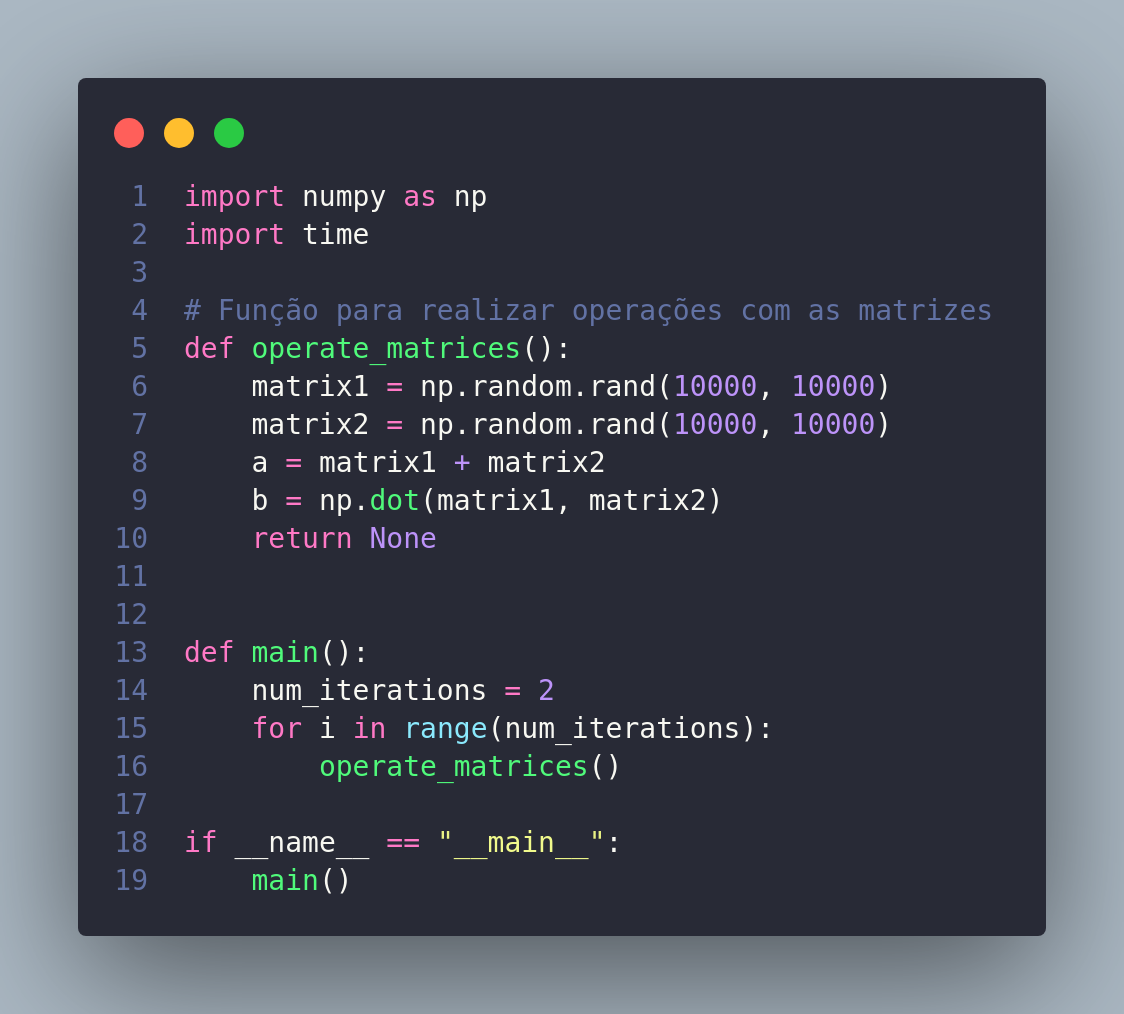
\includegraphics[width=0.6\textwidth]{swapy.png}
	\caption{heading}
	\label{fig:swapy}
\end{figure}


O código em questão (\ref{fig:swapy}) realiza operações com matrizes usando a biblioteca NumPy em Python. 
Abaixo, estão os principais pontos do código explicados:

\begin{itemize}[label=--]
    \item \textbf{Importação de Bibliotecas:}
    \begin{itemize}
        \item \texttt{import numpy as np}: Importa a biblioteca NumPy e a renomeia como \texttt{np} para facilitar o uso.
        \item \texttt{import time}: Importa a biblioteca \texttt{time} para medir o tempo de execução (embora essa funcionalidade não seja usada no código atual).
    \end{itemize}
    
    \item \textbf{Definição da Função \texttt{operate\_matrices}:}
    \begin{itemize}
        \item Gera duas matrizes aleatórias de tamanho \(10000 \times 10000\), denominadas \texttt{matrix1} e \texttt{matrix2}.
        \item Realiza duas operações com as matrizes:
        \begin{itemize}
            \item \texttt{a = matrix1 + matrix2}: Soma elemento por elemento das duas matrizes.
            \item \texttt{b = np.dot(matrix1, matrix2)}: Calcula o produto ponto a ponto das duas matrizes.
        \end{itemize}
        \item Retorna \texttt{None}.
    \end{itemize}
    
    \item \textbf{Função \texttt{main}:}
    \begin{itemize}
        \item Define o número de iterações como \texttt{num\_iterations = 2}.
        \item Realiza um loop \texttt{for} com \texttt{num\_iterations} chamando a função \texttt{operate\_matrices} em cada iteração.
    \end{itemize}
    
    \item \textbf{Condição \texttt{if \_\_name\_\_ == "\_\_main\_\_":}}
    \begin{itemize}
        \item Garante que o código dentro deste bloco seja executado apenas se o script for executado como um programa independente, não se for importado como um módulo.
        \item Chama a função \texttt{main()} para iniciar a execução do programa.
    \end{itemize}
\end{itemize}

% ---
\chapter{Conclusão}
\label{conclusao}


% ----------------------------------------------------------
% ELEMENTOS PÓS-TEXTUAIS
% ----------------------------------------------------------
\postextual
% ----------------------------------------------------------

% ----------------------------------------------------------
% Referências bibliográficas
% ----------------------------------------------------------
\bibliography{bibliografia}
% ---


% ----------------------------------------------------------
% Apêndices
% ----------------------------------------------------------

% ---
% Inicia os apêndices
% ---

% ----------------------------------------------------------
% Anexos
% ----------------------------------------------------------

% ---
% Inicia os anexos
% ---


\end{document}
